% !TeX spellcheck = en_US
% !TeX encoding = UTF-8
%%%%%%%%%%%%%%%%%%%%%%%%%%%%%%%%%%%%%%%%%%%%%%%%%%%%%%%%%%%%
\chapter{Stress Detection Methodology}


\begin{figure}[h]
	\centering
	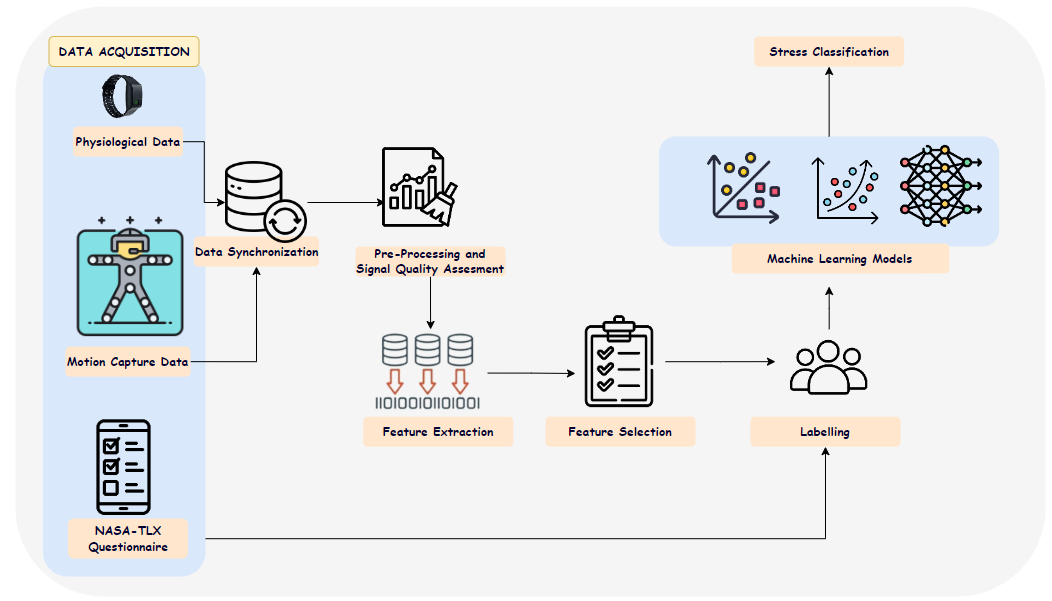
\includegraphics[width=\columnwidth]{images/Screenshot_5.png}
	\caption{Schematic of the experiment setup}
	\label{fig:netwrok}
\end{figure}

\section{Data Synchronization} \label{sec:Synchronization} \gls*{gptmo}
As previously eluded in section \ref{sec:expprot}, data synchronization is crucial to our experimental framework, ensuring the consistency
of data gathered from all the different sensors. In our setup, since the Empatica E4 wristband collects various physiological signals, including Blood Volume Pulse(BVP), Electrodermal Activity (EDA), Heart Rate (HR), and skin temperature at different frequencies as well as the motion capture system that tracks the participant's movements at a higher frequency. Given the varying sampling rates of these data sources, it's crucial to synchronize them to ensure they are comparable and accurate.

The Empatica E4 wristband samples at different rates for different signals: the Blood Volume Pulse (BVP) data is transmitted at 64Hz, while other metrics like EDA and temperature are transmitted at a lower rate of 4Hz. In contrast, the motion capture data, processed by the Motive software, is typically captured at a higher rate, around 120Hz. These discrepancies in sampling rates necessitate a careful synchronization approach.


Our synchronization strategy focuses on aligning diverse data streams to a unified frequency. Considering the need for detailed data and practical data processing constraints, we standardize all data streams to a frequency of 64Hz, matching the Blood Volume Pulse (BVP) rate from the Empatica E4. This standardization process involves downsampling the motion capture data, which originally records at a higher frequency of 120Hz. Simultaneously, for other signals like the Electrodermal Activity (EDA) and temperature, updating at a lower frequency of 4Hz, and acceleration data at 32Hz, we use a forward-filling approach, carrying their most recent values until an update occurs.

A specialized ROS node is responsible for this synchronization.  By using the BVP rate as the master reference, the node ensures that both physiological and motion data are synchronized in time. This alignment is key for an integrated and comprehensive analysis of the participant's responses, providing a dataset that accurately reflects both the physiological states and physical movements.

Once synchronized, the data is then published to a ROS topic, typically /aggregated\_data. This topic carries a comprehensive stream of information that combines detailed physiological measures with precise motion data. This rich dataset forms the foundation for subsequent phases of analysis in our study, such as feature extraction and stress detection.

\section{Pre-Processing} \gls*{gptmo}
Pre-processing is a crucial step in the analysis of data from physiological sensors and motion capture systems, as it prepares the raw data for subsequent processing and analysis phases. This section outlines the key aspects of pre-processing in our study.

\subsection*{Data Filtering} \label{sec:data_filtering}

In the pre-processing phase of our study, data filtering plays a crucial role in refining the quality of the signals gathered from the physiological sensors and motion capture systems. This step involves applying specific filtering techniques to the raw data to remove any unwanted data, thereby enhancing the signal's clarity and usability for further analysis.

The primary objective of data filtering is to isolate the significant aspects of the signal while eliminating any unwanted noise or interference. Depending on the nature of the signal and the type of noise present, different filtering methods are employed. For instance, we use N-th order Butterworth filters, which are effective in retaining the desired frequency range while attenuating frequencies outside this range. The Butterworth filter is known for its smooth frequency response and is particularly useful in physiological signal processing where preserving the integrity of the signal is crucial.

Each signal type dictates specific filter parameters like filter order, cutoff frequencies, and filter type (lowpass, highpass, or bandpass). This careful selection ensures the final signal is representative of the true physiological data crucial for accurate analysis.

\subsection*{Data Normalization}
Normalization is a critical step in data pre-processing aswell, particularly when dealing with signals of varying magnitudes or scales. Our approach involves applying a normalization process to each input signal, which standardizes the range of data values. This step is essential for comparing and combining data from different sensors effectively.

The method we use for normalization is primarily the 'z-score' method. This technique transforms the data to have a mean of zero and a standard deviation of one. By doing so, it ensures that each signal contributes equally to the analysis, irrespective of their original scale or distribution. This standardization is crucial for machine learning models, as it enhances algorithm performance and prevents any single feature from dominating due to its scale.

Normalization also aids in mitigating the impact of outliers, as it brings all data points onto a common scale, making them more suitable for analysis.

\begin{comment}
\subsection*{Peak Detection}
Peak detection is a method used to identify significant local maxima (peaks) and minima (troughs) in the data, which can represent important events or changes. In the context of stress detection, for instance, identifying peaks in heart rate or GSR signals can be indicative of moments of heightened stress or arousal. Efficient peak detection algorithms are crucial for accurately identifying these critical points in the data. Analyzing the frequency and intensity of these peaks can provide valuable insights into the physiological response patterns of the participants, such as the frequency of stress episodes or the degree of response to different stimuli.
\end{comment}

\subsection*{Signal Quality Assessment}
\label{sec:signal_quality_assessment}

Signal quality assessment is an integral part of the preprocessing phase to ensure the reliability and accuracy of data collected from sensors, which is fundamental for accurate analysis. Various methods are employed to assess the quality of signals, each targeting specific types of anomalies or artifacts.

\paragraph{Detection of Clipped Segments:}
This method involves identifying segments in the signal that are clipped or truncated. Clipping often occurs when the signal amplitude reaches the sensor's recording capacity limits. By setting thresholds for positive and negative clipping, the method detects and marks these segments, facilitating their exclusion or correction .

\paragraph{Detection of Flatline Segments:}
This method identifies flatline segments where the signal shows minimal variation over a period. Such segments can indicate sensor displacement or malfunction. The method identifies these periods by assessing the duration of flatness and the threshold for change in signal amplitude, helping exclude non-physiological data from the analysis.


Each method plays a crucial role in verifying the integrity of the signal data. Identifying and addressing issues like clipping, flatlining, and inconsistent patterns, signal quality assessment ensures that subsequent data analysis stages are based on accurate and reliable data.



\subsection*{Baseline Correction}
\label{sec:baseline_correction}

Baseline correction forms a pivotal part of our data normalization strategy, particularly tailored for participant-specific physiological data. This approach is centered around the concept of adjusting the data relative to each participant's baseline physiological state, typically captured during a rest period prior to the experimental tasks. This preparatory measure establishes a reference point against which subsequent physiological responses are compared.
In the baseline correction process, we begin by computing the average values of physiological signals recorded during the baseline phase before the start of the experiment. This baseline phase is critical as it represents a period of rest where the participant's physiological state is unaffected by experimental stressors. By establishing this baseline, we are able to set a reference point that reflects the participant's normal physiological state. Subsequently, we adjust the data points collected during the active phases of the experiment relative to these baseline averages. This adjustment is a normalization process that centers the data around a personalized zero point, effectively accounting for individual physiological variations. The core advantage of baseline correction lies in its ability to mitigate the influence of inter-individual variability on the physiological measurements. Since each participant's baseline state can vary significantly due to factors like inherent physiological differences, stress levels, and environmental conditions, normalizing data against this baseline ensures a more accurate and personalized assessment of stress responses.
This method ensures that the changes observed in the physiological data during the experiment are indicative of the participant's response to the experimental conditions, rather than being a reflection of their baseline physiological state.

\subsection*{Signal Segmentation}
\label{sec:signal_segmentation}
In our research, the segmentation of physiological and motion capture data into windows was a crucial part of the preprocessing. This process involved breaking down the continuous data streams into smaller, manageable windows for detailed analysis. The selection of window size and step size was critical, and was tailored based on the characteristics of the signal and the objectives of our analysis.

The window size was carefully chosen to capture relevant physiological and behavioral patterns within each segment, balancing the need to encapsulate meaningful data against the computational demands of processing. The step size determined the overlap between these windows, ensuring continuity and that no significant transient events were missed.

Accounting for the sampling rate of each signal was vital in customizing the segmentation process appropriately. This flexible approach was key to accommodating different types of signals, ensuring that the window size was appropriate for the length of the signal and that the segmentation parameters were compatible with each signal's nature.

Segmenting data into windows enabled us to convert the ongoing data streams into a format suitable for comprehensive analysis. This structured approach facilitated subsequent computational processes, including feature extraction and pattern recognition, essential for robust stress detection and analysis. This method of using windows in data segmentation is fundamental in ensuring that each part of the continuous data stream is analyzed effectively, allowing for a thorough understanding of stress indicators within the dataset.

\section{Feature Extraction} \gls*{gptmo}
Feature Extraction and Selection play a pivotal role in the effectiveness of machine learning models, especially in the context of human stress recognition. Feature extraction involves deriving meaningful attributes from the raw data collected. The type of features extracted can vary widely, including statistical features, time-domain, frequency-domain, as well as linear versus non-linear features.

The complexity of these features can range from basic statistical measures like mean, median, minimum, and maximum, to more intricate features based on specific data modalities. Each sensor used in stress detection may yield a unique set of features, contributing to the overall data analysis and model accuracy. The selection and application of these features are crucial, as they directly impact the classification stage, ultimately influencing the model's performance in stress recognition.

\subsection{EDA-Electrodermal Activity}

Electrodermal Activity (EDA), also known as galvanic skin response (GSR), is a sensitive measure of emotional and physiological arousal. It primarily consists of two components: tonic (Skin Conductance Level, SCL) and phasic (Skin Conductance Response, SCR).As explained in Section \ref*{subsec:EDAtheory} the tonic component represents baseline levels of skin conductance, reflecting slow changes in arousal state. The phasic component, on the other hand, captures rapid fluctuations in response to specific stimuli or events.


After the usual process of filtering and normalizing the signal aswell checking the quality of the signal we first decompose the EDA signal into its tonic and phasic components using continuous decomposition analysis. This process allows us to separately analyze the steady-state (SCL) and transient (SCR) aspects of skin conductance.
The decomposition is typically carried out using highpass filtering techniques, ensuring that each component accurately represents the underlying physiological processes.
\begin{figure}[hb]
	\centering
	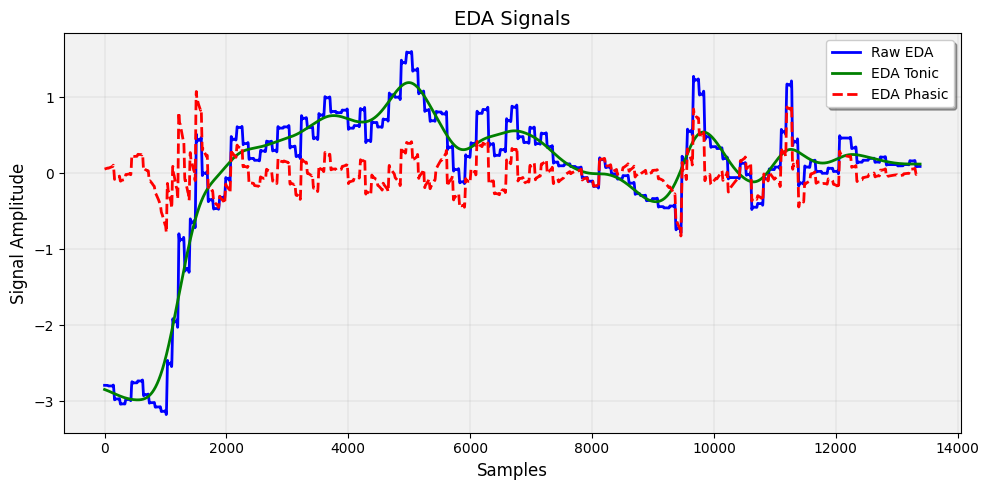
\includegraphics[width=\columnwidth]{images/eda.png}
	\caption{EDA}
	\label{fig:eda sig}
\end{figure}

We conducted a comprehensive review and comparison of various EDA features, ultimately selecting those most relevant to our research objectives. This meticulous selection process, influenced by a thorough examination of nearly 40 distinct EDA features as outlined by previous studies \textcite{EDAFeatures}, enabled us to tailor our feature set.

From the decomposed EDA data, a variety of time domain statistical features can be extracted. These include mean ($\mu$), standard deviation ($\sigma$), coefficient of variance (CV), variance ($\sigma^2$), and kurtosis ($\beta$) from the phasic component.

Mean ($\mu$) provides a measure of the central tendency of the SCR amplitudes.
Standard deviation ($\sigma$) and variance ($\sigma^2$) capture the variability or dispersion around the mean.
The coefficient of variance (CV) offers a normalized measure of dispersion relative to the mean.
Kurtosis ($\beta$) evaluates the peakedness or flatness of the distribution of SCR amplitudes.

In addition to time-domain features, we analyze the EDA signal in the frequency domain. Furthermore, frequency-domain features like spectral power in specific bands (f1sc, f2sc, f3sc) and the overall energy and entropy of the signal gave us a spectrum-based view of the EDA responses. By analyzing these features, we could discern patterns and rhythms in the EDA that are not immediately apparent in the time-domain.


Detecting and analyzing peaks in the phasic component (SCRs) is crucial. Peak amplitude, frequency, and their inter-relationships can be strong indicators of emotional and cognitive stress responses.

By examining both tonic and phasic components, we can understand the sustained arousal level (SCL) and the specific responses to stimuli (SCR). The correlation between these components can provide valuable insights into how sustained stress levels influence responses to immediate stimuli.
From the tonic component, which encapsulates the underlying level of arousal, we calculated the mean, capturing the central tendency over time, and the standard deviation, offering insights into the variability around this mean. The maximum and minimum values, along with the range, provided us with the extremes of the EDA signal, painting a picture of the breadth of responses.

From the phasic component, we focused on the Skin Conductance Responses (SCRs) to discern more rapid changes associated with specific stimuli. We extracted features like SCR amplitude, which reflects the intensity of the response, and the frequency of these SCRs, indicating how often these responses occur. The kurtosis of SCR amplitudes, a measure of the 'tailedness' of the distribution, gave us an understanding of how peaked or flat the distribution of responses was, while the skewness indicated any asymmetry, offering clues about the predominant direction of the response distribution.

We also looked at the root mean square (SCR RMS), which is a measure of the signal's magnitude, and the arc length (SCR Arc Length), providing a summative measure of the signal's complexity over a given period. The integral of the SCR signal (SCR Integral) was calculated to understand the total magnitude of these phasic responses over time. These features, alongside others like SCR momentum, which is akin to the second moment of the distribution, provided a comprehensive statistical breakdown of the phasic EDA signals.

\textcite[]{EDAFeatures}  we reviewed and compared amlost 40 different EDA features, the features extracted selected with the help of this.

\subsection{Body Features}
Since we captured human motion using the motion capture system, we selected 13 key points from the 25 marker points used by the system, focusing on the upper body. The chosen points were Hip, Ab, Chest, Neck, Head, Left Shoulder (LShoulder), Left Upper Arm (LUArm), Left Forearm (LFArm), Left Hand (LHand), Right Shoulder (RShoulder), Right Upper Arm (RUArm), Right Forearm (RFArm), and Right Hand (RHand). These points were strategically selected to comprehensively capture upper body movements. The arrangement of these points is depicted in Fig \ref{fig:human}

\begin{figure}[h]
	\centering
	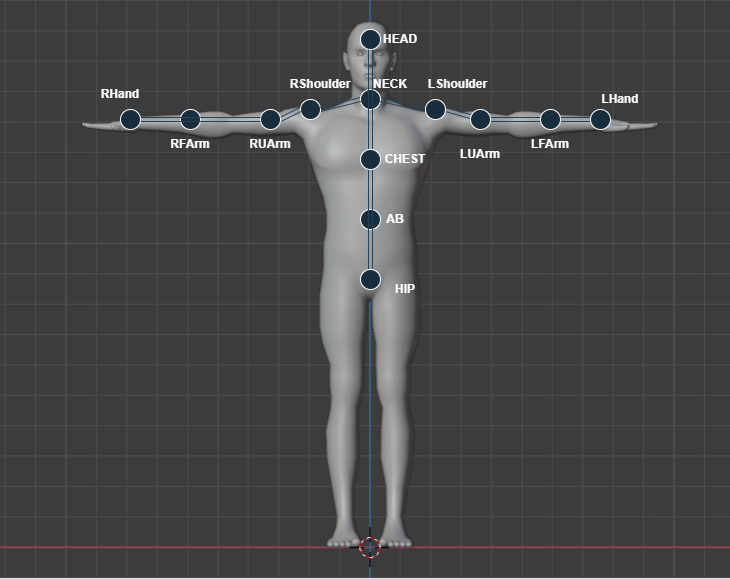
\includegraphics[width=0.8\columnwidth]{images/human.png}
	\caption{13 points from the motion capture} 
	\label{fig:human}
\end{figure}


%\textcite[postnote]{HARRIGAN19851161} HARRIGAN19851161
\subsection*{Self Touching} 
Previous studies, such as the one referenced in \textcite{10.1371/journal.pone.0043571}, indicate that body posture and body language can be valuable indicators of stress. In line with this, we also explored body language cues such as self-touching, which \textcite{HARRIGAN19851161}suggests can be indicative of negative affect, such as anxiety or discomfort. Specifically, we focused on face and head touching as potential stress indicators.

To determine if a person is touching her face, we compute the hand-head and the hand-neck distances. If one of these distances is below a given threshold, we consider that the person is face touching. The number of occurrences (FTC) and the average duration (FTMD) of these face touching events are used as features. 

To determine gestures such as face touching, \texttt{/tf} data, which typically includes the position and orientation of each joint in space, can be utilized to calculate the distance between any two points. For example, if you have the coordinates of the right hand (\texttt{RHand}) and the head (\texttt{HEAD}), you can compute the Euclidean distance between these two points at each time frame to detect when the hand is close enough to the head to indicate potential face touching.

Let's define the 3D coordinates for the right hand and head at time $t$ as:
\begin{itemize}
\item $P_{\text{RHand}}(t)$ for the position of the right hand at time $t$, with coordinates $(x_{\text{RHand}}(t), y_{\text{RHand}}(t), z_{\text{RHand}}(t))$,
\item $P_{\text{HEAD}}(t)$ for the position of the head at time $t$, with coordinates $(x_{\text{HEAD}}(t), y_{\text{HEAD}}(t), z_{\text{HEAD}}(t))$.
\end{itemize}

The distance between the right hand and the head at time $t$ is then calculated with the formula:

\begin{equation}
D_{\text{RHand-HEAD}}(t) = \sqrt{(x_{\text{RHand}}(t) - x_{\text{HEAD}}(t))^2 + (y_{\text{RHand}}(t) - y_{\text{HEAD}}(t))^2 + (z_{\text{RHand}}(t) - z_{\text{HEAD}}(t))^2}
\end{equation}

If this distance, $D_{\text{RHand-HEAD}}(t)$, is less than a certain threshold, denoted as $\theta$, it suggests that the right hand is in proximity to the head, indicating potential face touching.

To determine the occurrence of face touching, you would track when this distance becomes less than the threshold $\theta$ and also ensure that the hand remains within this threshold for a certain duration to count as an occurrence. The distance for the left hand can be calculated in a similar manner.

To compute the number of occurrences (\texttt{FTC-Face Touching Count}) and the average duration (\texttt{FTMD-Face Touching Mean Duration}) of face touching is shown in Algorithm \ref{alg:face_touching}.

    \begin{algorithm}
        \caption{Face Touching Detection}
          \label{alg:face_touching}
        \begin{algorithmic}[1]
          \Require{Set of time-stamped positions from the \texttt{/tf} topic, Threshold distance $\theta$}
          \Statex
          \Function{DetectFaceTouching}{}
            \State Initialize $FTC \gets 0$ \Comment{Occurrences of face touching}
            \State Initialize $TotalDuration \gets 0$ \Comment{Total duration of face touching events}
            \State Initialize $FTMD \gets 0$ \Comment{Mean duration of face touching events}
            
            \For{each time stamp $t_i$ in \texttt{/tf} topic}
              \State Calculate $D_{RHand-Head}(t_i)$ and $D_{LHand-Head}(t_i)$
              
              \If{$D_{RHand-Head}(t_i) < \theta$ \textbf{or} $D_{LHand-Head}(t_i) < \theta$}
                \State Start duration counter
                \State $FTC \gets FTC + 1$
              \EndIf
              
              \If{either distance exceeds $\theta$}
                \State Stop duration counter
                \State Add duration to $TotalDuration$
              \EndIf
            \EndFor
            
            \If{$FTC > 0$}
                \State $FTMD \gets \frac{TotalDuration}{FTC}$ \Comment{Calculate mean duration}
            \EndIf
            \State \textbf{return} $FTC$, $FTMD$
          \EndFunction
        \end{algorithmic}
      \end{algorithm}

      
\subsection*{Sudden Movement }
\label{subsec:sudden_movement_analysis}

\textcite{hyperactivity} suggested another way in which motion data can be used to assess stress.
Sudden movements, or abrupt changes in body motion, can be indicative of stress responses. These movements are characterized by significant deviations from a person's regular movement patterns and can be quantitatively assessed using motion capture data. The following equations describe the computational process used to analyze sudden movements and infer stress.

\begin{equation}
m_j^k = \sum_{i=0}^{\tau-1} d_j^{k-i,k-i-1}
\label{eq:movement_joints}
\end{equation}

Equation~\ref{eq:movement_joints} defines the movement of the \( j^{th} \) joint within a time window \( \tau \) as the sum of the displacements between consecutive frames. 

\begin{equation}
\Delta_j^k = m_j^k - \mu_j
\label{eq:deviation_baseline}
\end{equation}

In Equation~\ref{eq:deviation_baseline}, \( \Delta_j^k \) represents the deviation of the \( j^{th} \) joint's movement from its baseline mean motion \( \mu_j \), calculated during a calibration phase.

\begin{equation}
a_j^k = 
\begin{cases} 
  \frac{\Delta_j^k}{\sigma_j} - 1 & \text{if } \Delta_j^k > \sigma_j \\
  0 & \text{otherwise}
\end{cases}
\label{eq:activity_evaluation}
\end{equation}

Equation~\ref{eq:activity_evaluation} assesses the activity level \( a_j^k \) for the \( j^{th} \) joint, taking into account the standard deviation \( \sigma_j \) as a threshold for sudden movement.

\begin{equation}
a_k = \min \left( 1, \frac{1}{N} \sum_{j=1}^{N} a_j^k \right)
\label{eq:descriptor_sudden_movement}
\end{equation}

Finally, Equation~\ref{eq:descriptor_sudden_movement} calculates the overall level of sudden movement at time instance \( k \) by averaging the activities across all joints, thus providing a descriptor of hyperactivity or sudden movement.

This method allows for a comprehensive analysis of the motion data to identify periods of high activity that may correlate with stress responses.


While our study focused on the analysis of upper body movements for stress detection, it is important to note that other bodily cues can also be significant indicators of stress or anxiety. One such example is the rapid tapping or bouncing of one's feet, which is often a subconscious response to nervous energy or unease. Such movements are typically a form of self-soothing behavior that occurs when an individual is experiencing discomfort or stress.

Unfortunately, due to the scope of our motion capture system setup, we restricted our tracking to the upper body and therefore could not capture lower body movements, such as foot tapping or leg bouncing. These actions could potentially provide additional insights into a participant's stress levels and offer a more comprehensive understanding of physical stress responses.

Including lower body data in future studies could enhance the detection and analysis of stress indicators, allowing for a fuller picture of the physiological and behavioral state of an individual under stress. This would enable us to capture a wider range of stress-related behaviors and potentially increase the accuracy and reliability of stress detection in real-time scenarios.
\section{Classification /Stress Detection/}
